\documentclass{article}

\usepackage[margin=3cm]{geometry}
\usepackage{polyglossia}
	\setmainlanguage{english}
\usepackage{amsmath}
\usepackage{amssymb}
\usepackage{siunitx}
\usepackage{float}
\usepackage{booktabs}
\usepackage{subcaption}
\usepackage{graphicx}
\usepackage{xcolor}
\usepackage{listings}
    \lstset{language=Python,
	basicstyle=\footnotesize\ttfamily,
	breaklines=true,
	framextopmargin=50pt,
	frame=bottomline,
	backgroundcolor=\color{white!85!black},
	commentstyle=\color{blue},
	keywordstyle=\color{red},
	stringstyle=\color{orange!80!black}}
\usepackage{tikz}

\title{Computational Physics - Exercise 6}
\author{Maurice Donner \and Lukas Häffner}

\begin{document}

\maketitle
\newpage

\section*{2 - Population dynamics}

Look at the equation
\begin{align}
    \frac{DN}{dt} = rN(1-N/K)- \frac{BN^2}{A^2 +N^2}
    \label{problem}
\end{align}
Where all parameters $r$, $K$, $A$ and $B$ are positive and have the
following dimensions:
\begin{align}
    [r] = [B] &= \frac{1}{\text{time}} \\[0.3cm]
    [N] = [A] = [K] &= 1
\end{align}
Defining dimensionless versions for N and t
\begin{align}
    n &= N/A \\
    \tau &= B \cdot t
\end{align}
Equation \ref{problem} can be rewritten in a dimensionless form:
\begin{align}
    \frac{dn}{d\tau} = \frac{r}{B} n \left( 1 - \frac{An}{K} \right) -
    \frac{n^2}{A(1+n^2)} 
\end{align}
Defining \( r/B \equiv c \) we can rewrite this equation to
\begin{align}
    \frac{dn}{d \tau} = - \frac{A}{K} n^3 + n^2 - \left( \frac{1}{Ac} +
	\frac{A}{K} \right) n + 1
\end{align}
Knowing that \( K/A = \frac{15}{2} \), we now plot a set of functions
(by varying \( Ac \)) in order to search for stationary points. For that,
we write a short program to search for roots:

\begin{lstlisting}
def countzero(arr):
    counter = 0
    sign = np.sign(arr[0])
    for i in range(len(arr)):
        if(np.sign(arr[i]) != sign):
            sign = sign*(-1)
            counter += 1
    return counter
\end{lstlisting}

With that, its possible to create two diagrams that select between solutions
with three stationary points and one stationary point:

\begin{lstlisting}
c1 = ([])
c3 = ([])

for c in crange:
    roots = countzero(cubic(xaxis,c))
    if roots == 3:
        plt.subplot(211)
        plt.plot(xaxis,cubic(xaxis, c),color='green',linewidth=1)
        c3.append(c)
        plt.title('Three Stationary Points')
    if roots == 1:
        plt.subplot(212)
        plt.plot(xaxis,cubic(xaxis, c),color='black',linewidth=1)
        plt.title('One Stationary Point')
        c1.append(c)
\end{lstlisting}

The result is the following:
\begin{figure}[H]
\centering
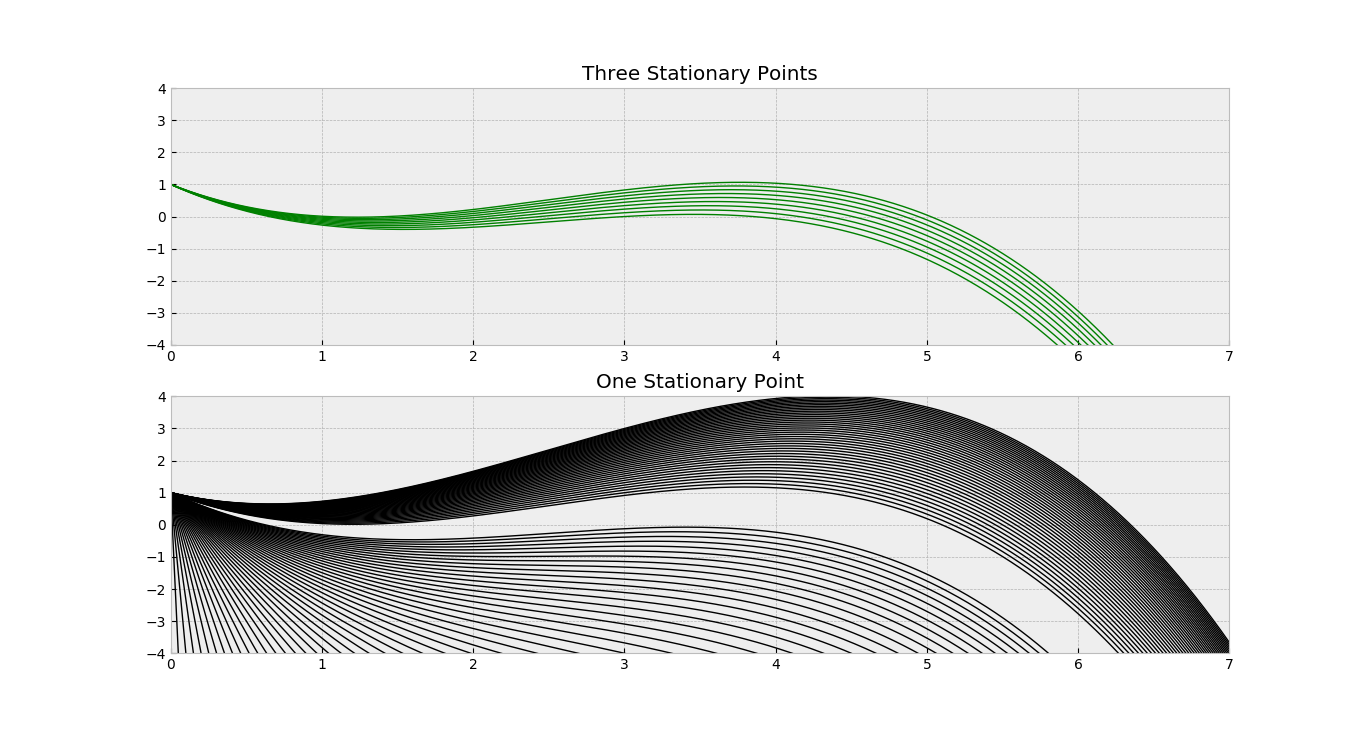
\includegraphics[width=.77\textwidth]{Stationary.png} 
\caption{Determining Stationary Points for different Ac} 
\end{figure}

To check if the points are stable, one has to examine the area around the point.
Lies the point in an upwards slope, it is unstable. Otherwise, it is stable.
In case of a saddle point, no definite answer can be made.\\
To check if a point is stable or not, all we need to do, is to check if the
sign in our \texttt{countzero}-Function changes from -1 to 1 (unstable) or from
1 to -1 (stable):

\begin{lstlisting}
def countzero(axis, arr, c):
    counter = 0
    sign = np.sign(arr[0])
    for i in range(len(arr)):
        if(np.sign(arr[i]) != sign):
            if (sign == 1): #Check if stable
                print('point at x = ', round(axis[i],2), 'for c = ', c, ' is stable')
            else:
                print('point at x = ', round(axis[i],2), 'for c = ', c, ' is unstable')
            sign = sign*(-1)
            counter += 1
    return counter
\end{lstlisting}

We now know that most of the points are stable. The only unstable points are the
ones between two stable solutions in functions with 3 stationary points:

\begin{table}[h]
    \centering
    \begin{tabular}{lcc}
	\toprule 
	\( Ac \) & x \\ \midrule 
	0.5 & 3.01 \\ 
	0.51 & 2.68 \\ 
	0.52 & 2.45 \\ 
	0.53 & 2.26 \\ 
	0.54 & 2.09 \\ 
	0.55 & 1.93 \\ 
	0.56 & 1.78 \\ 
	0.57 & 1.63 \\ 
	0.58 & 1.44 \\ 
	\bottomrule 
    \end{tabular}
    \caption{Unstable stationary points}
\end{table}

\end{document}

